\documentclass[a4paper,ngerman,landscape,30pt]{scrartcl}

\usepackage[utf8]{inputenc}
\usepackage{arabtex}
\usepackage{amsmath}

\usepackage[ngerman]{babel}
\usepackage{hyperref}

\usepackage{graphicx}

\usepackage[protrusion=true,expansion=true]{microtype}

\usepackage{lmodern}
\usepackage{tabto}

\setlength\parskip{\medskipamount}
\setlength\parindent{0pt}

\usepackage{geometry}
\geometry{tmargin=1.5cm,bmargin=1.0cm,lmargin=2.5cm,rmargin=2.5cm}

\pagestyle{empty}

\begin{document}

\newcommand{\page}[1]{
  \begin{center}
    \Huge\sffamily
    #1%
    \vfill
    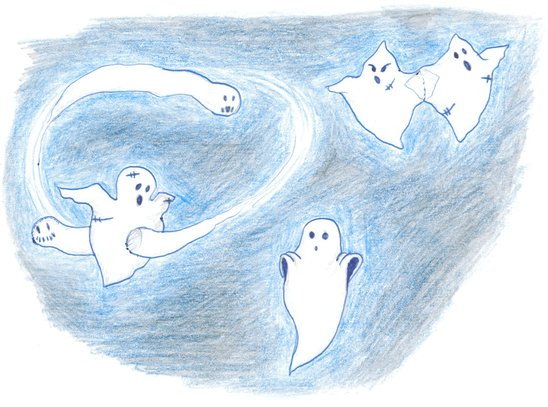
\includegraphics[scale=2]{../skript2/phantome-klein}
  \end{center}
  \newpage
}

\page{%
  \textbf{Simpliziale Mengen} sind Bastelanleitungen für topologische
  Räume.
}

\page{%
  \scalebox{3.8}{%
    \RL{%
    al-`ilmu al-^gabri al-ttamA_tuliyi
    }}
}

\page{%
  Mit \textbf{Garben}
  kann man effizient lokale Daten organisieren.
}

\page{%
  Wichtig sind \textbf{Beziehungen}
  zwischen Objekten.
}

\page{%
  \textbf{Adjunktionen} \\ sind überall.
}

\page{%
  \textbf{Komplexe} sind gut,
  \textbf{Kohomologie} ist schlecht.
}

\page{%
  Mit \textbf{abgeleiteten Funktoren}
  kann man Nichtexaktheit messen.
}

\page{%
  In abelschen Kategorien:
  \begin{align*}
    \textbf{Bild} &= \textbf{Kobild}
  \end{align*}
}

\page{%
  \textbf{Funktoren} bewahren
  Kommutativität.
}

\page{%
  Nützlich das
  \textbf{Yoneda-Lemma} ist.
}

\page{%
  Eine \textbf{Prägarbe} ist eine Art
  ideelles Objekt.
}

\page{%
  $\boldsymbol{\Delta}$ enthält den
  \textbf{wandelnden Monoid}.
}

\page{%
  Ich mach' \\ \textbf{nicht immer} \\ Algebra \ldots
}

\page{%
  \ldots aber wenn, dann \textbf{homologische}!
}

\end{document}
